\chapter{Relative Efficiency of Decoupled Flow Solver}
\label{chapter-eight}

At this point, the reacting gas adjoint in FUN3D has been utilized to obtain
sensitivity information needed to drive design optimization, and the
sensitivities of the fully coupled scheme have been validated against
finite-difference derivatives with a complex step for accuracy.  A key point of
this study is to demonstrate the increase computational efficiency and relative
memory saving of using a decoupled variable set for the flow and adjoint
solvers, instead of a fully coupled variable set.  This chapter details the
benefits of applying the decoupled flow solver over the fully coupled solver for
a variety of test cases, including the annular jet demonstration problem.

\section{5 km/s Flow over Cylinder}
\label{sec:5-kps-cylinder}

Demonstrating the improved efficiency in cost and memory required to utilize the
decoupled scheme, and that both the fully coupled and decoupled approaches
converge to the same result, a grid convergence study was conducted on a simple
cylinder geometry (radius 0.5 m).  Due to the presence of strong shocks in blunt
body flows, it was advantageous to generate structured-type grids to preserve
grid alignment with the bow shock. A 50$\times$50, 100$\times$100, and
200$\times$200 family of grids were adapted using the adaptation capability in
FUN3D\cite{adaptation} to produce shock-aligned grids. These grids serve as a
surrogate for conducting a grid convergence study, in that differences observed
between the decoupled and fully coupled schemes decrease as the average mesh
spacing decreases.  These grids are unstructured, consisting totally of
hexahedra elements with a single cell in the spanwise direction, and the
50$\times$50 grid is shown in Figure \ref{grid}.  The cell elements of these
grids were also subdivided into tetrahedral elements, and it was verified that
there are no issues with a true unstructured grid topology.  The free stream
conditions used were $V_{\infty} = 5000\ m/s$, $\rho_{\infty}=0.001\ kg/m^3$,
and $T_\infty = 200\ K$.  Several chemical kinetics models were used, including
a 5-species model with 5 reactions, an 11-species model with 22 reactions, and
an 18-species model with 29 reactions.  All cases were run in thermal
equilibrium, with a one-temperature model.

%------------------------------------------------------------------------------%
\begin{figure}[h]
	\centering
  \adjincludegraphics[width=0.8\textwidth,trim={0 4cm 0 4cm},clip]{figures/scitech/grid}
	\caption{50$\times$50 cylinder grid.}
  \label{grid}
\end{figure}
%------------------------------------------------------------------------------%

\subsection{Cylinder - Verification of Implementation}

In order to be valid, the decoupled scheme must yield converged solutions that
are nearly identical to those of the fully coupled system. To quantitatively
assess this, we compare the predicted surface pressure, surface temperature, and
the species composition on the stagnation line for both schemes.  Figure
\ref{pq} shows the predicted quantities on the 100$\times$100 grid, for species
mixture of N, $\text{N}_2$, O, $\text{O}_2$, and NO with five reactions. All
results are indeed nearly identical, with temperature and pressure matching
discretely to eight digits and the species mass fractions on the stagnation line
matching to four digits.  This difference was further reduced on the finest grid
level of 200$\times$200, suggesting that both schemes converge to the same
solution with grid refinement.
%------------------------------------------------------------------------------%
\begin{figure}[h!]
  \captionsetup[subfigure]{position=b}
  \centering
  \subcaptionbox{Surface pressure}{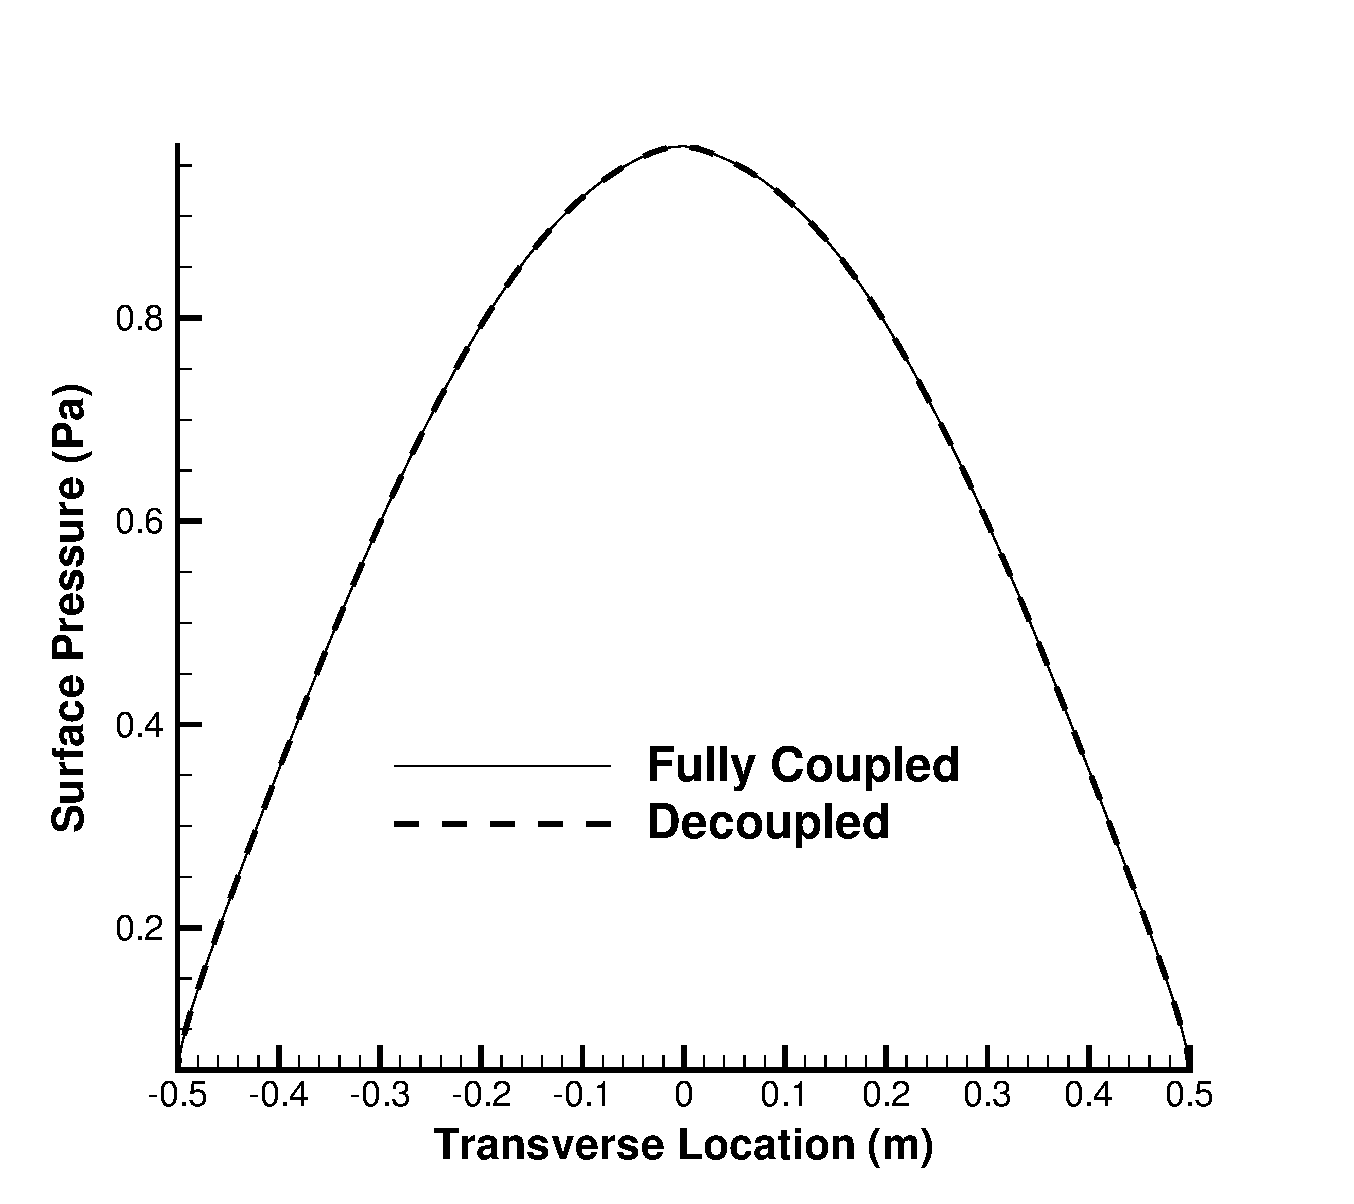
\includegraphics[width=0.3\linewidth]{figures/scitech/surface_pressure}}
  \subcaptionbox{Surface temperature}{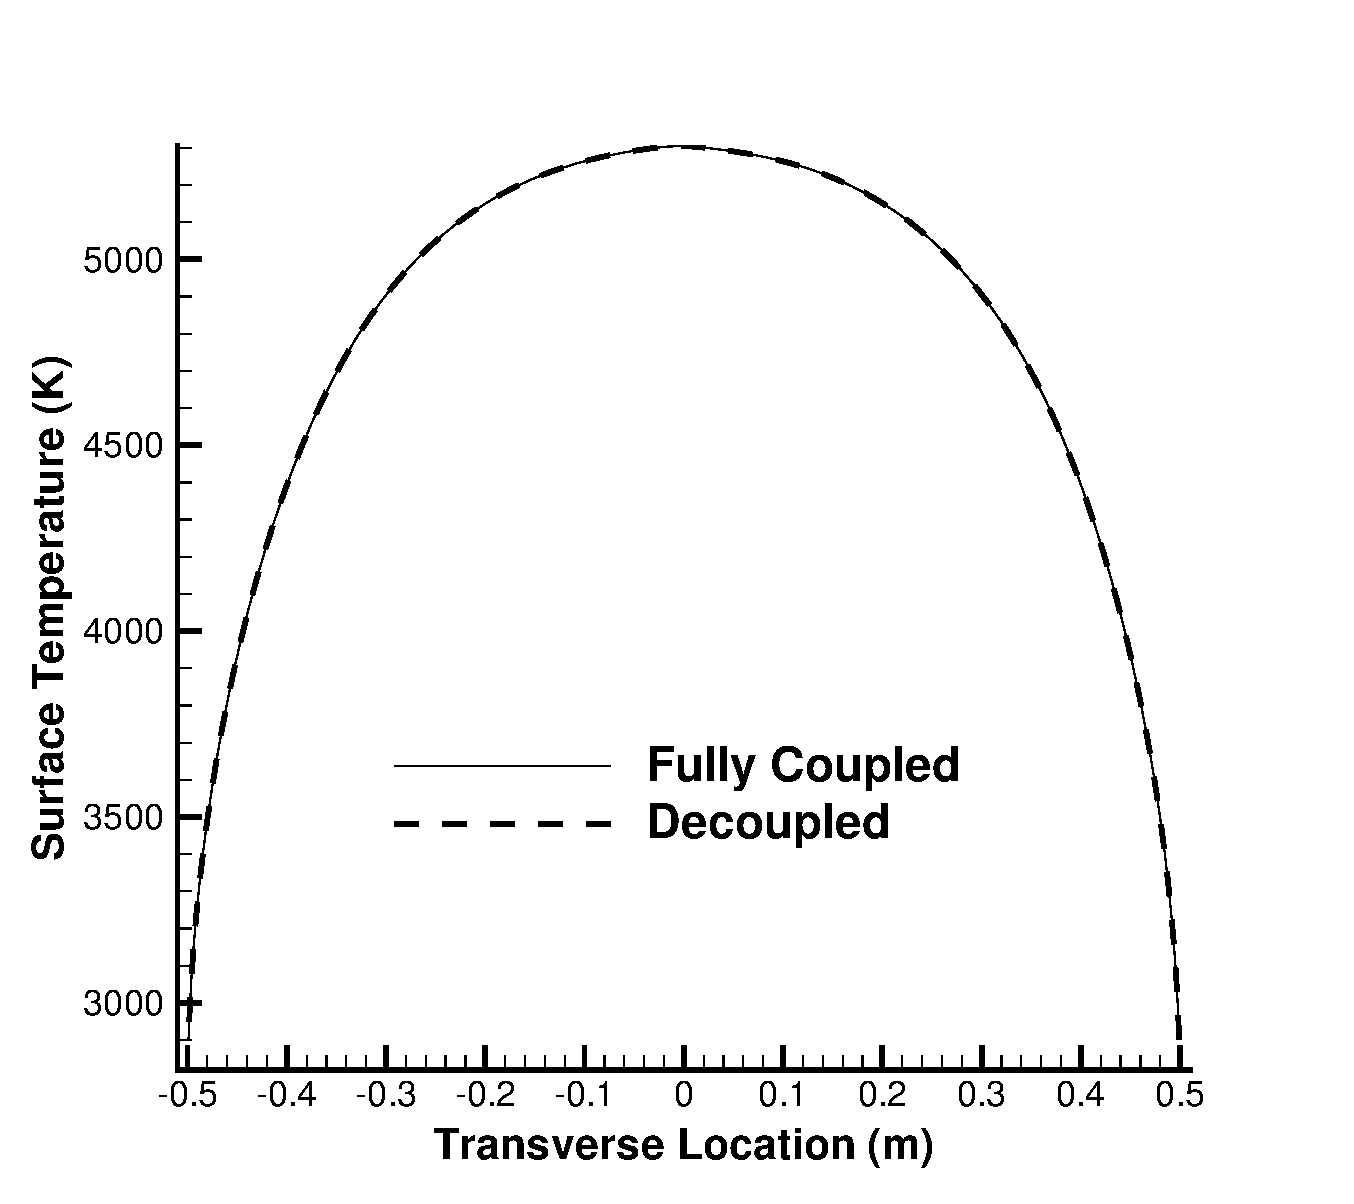
\includegraphics[width=0.3\linewidth]{figures/scitech/surface_temperature}}
  \subcaptionbox{Mass fractions on stagnation line}{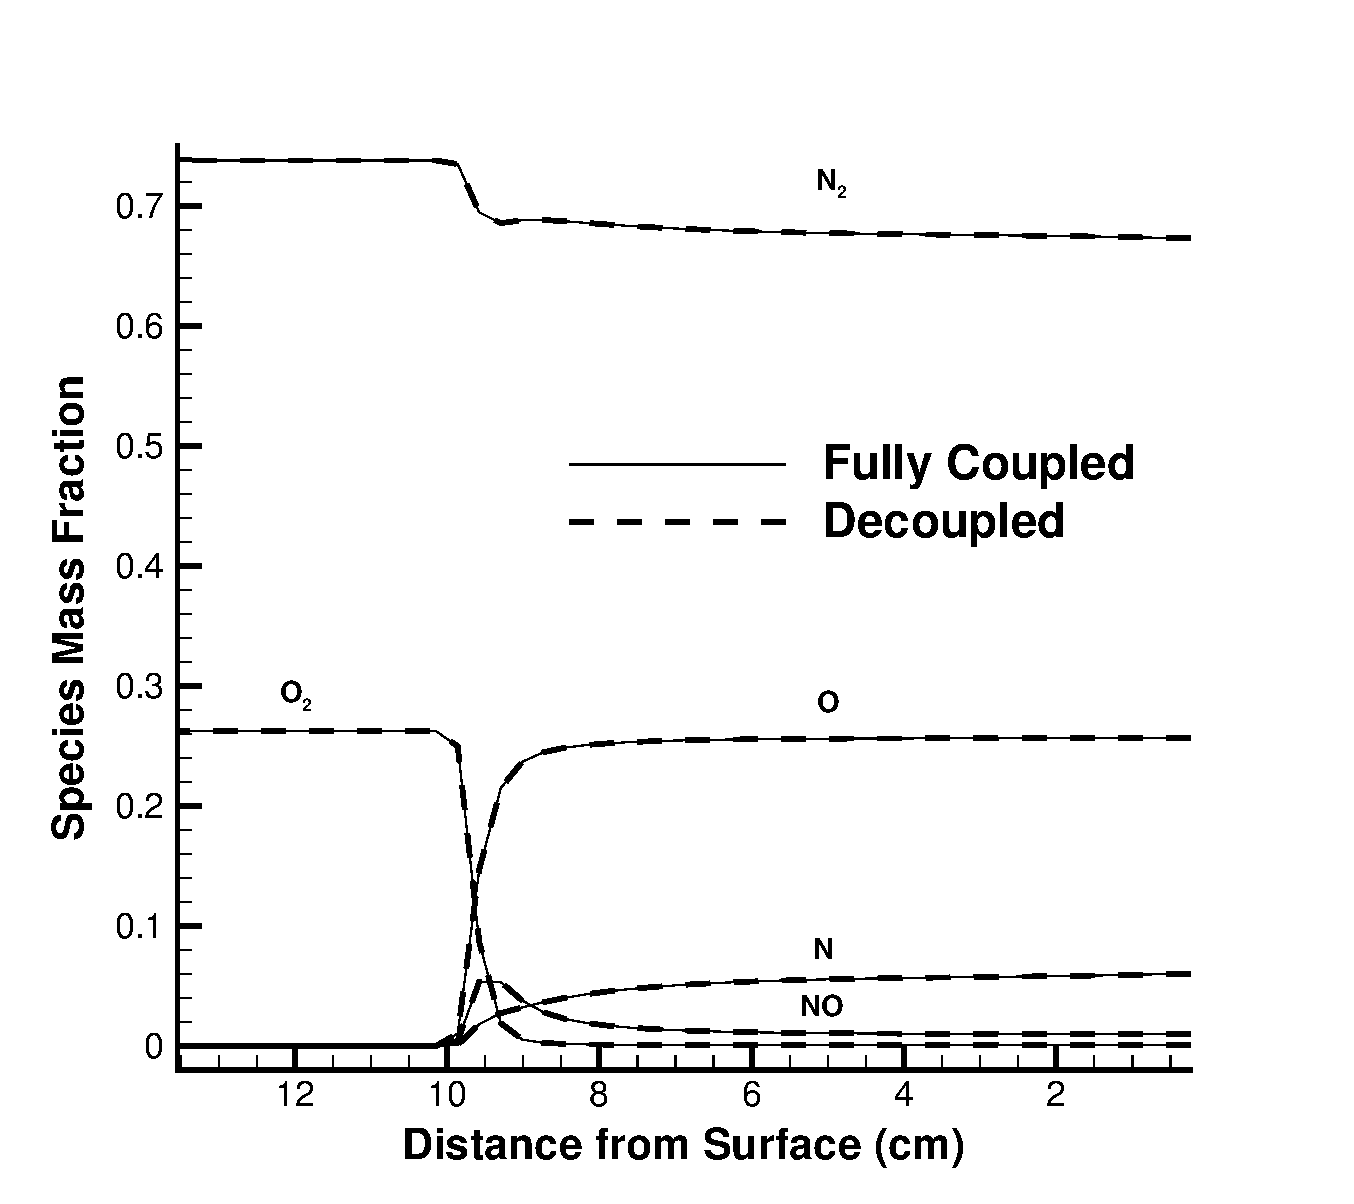
\includegraphics[width=0.32\linewidth]{figures/scitech/stag_line_mf}}
	\caption{Cylinder predicted quantities.}
	\label{pq}
\end{figure}
%------------------------------------------------------------------------------%

\subsection{Cylinder - Memory Cost}

In order to determine the required memory of the decoupled scheme compared
to the fully coupled scheme, a convergence study was conducted using
Valgrind\cite{valgrind} to determine the memory actually allocated by FUN3D for
an increasing number of species.  
Figure \ref{mem_req} shows that the relative memory cost converges asymptotically to
$\sim$1/4, which is nearly twice the predicted value of 1/7.  For the
implementation of FUN3D, this is correct because the off-diagonal entries are
reduced from double to single precision.  Each structured grid node has six
neighboring nodes, with the exception of those at the boundary.  Because each of
these six neighboring nodes yields single precision, off-diagonal Jacobian
elements, 
%------------------------------------------------------------------------------%
\begin{equation} 
  N_{nz} = \frac{6N_{nodes}}{2} = 3N_{nodes}
  \label{f3d_off_diag} 
\end{equation} 
%------------------------------------------------------------------------------%
Substituting \eref{f3d_off_diag} into \eref{mem_req_eq}, the relative memory
cost is:
%------------------------------------------------------------------------------%
\begin{equation} 
  Relative\ Memory\ Cost = 
  \frac{N_{nodes}}{N_{nodes} + N_{nz}} =
  \frac{N_{nodes}}{N_{nodes} + (3N_{nodes})}=\frac{1}{4}
\end{equation}
%------------------------------------------------------------------------------%
%------------------------------------------------------------------------------%
\begin{figure}[h] 
  \begin{center} 
    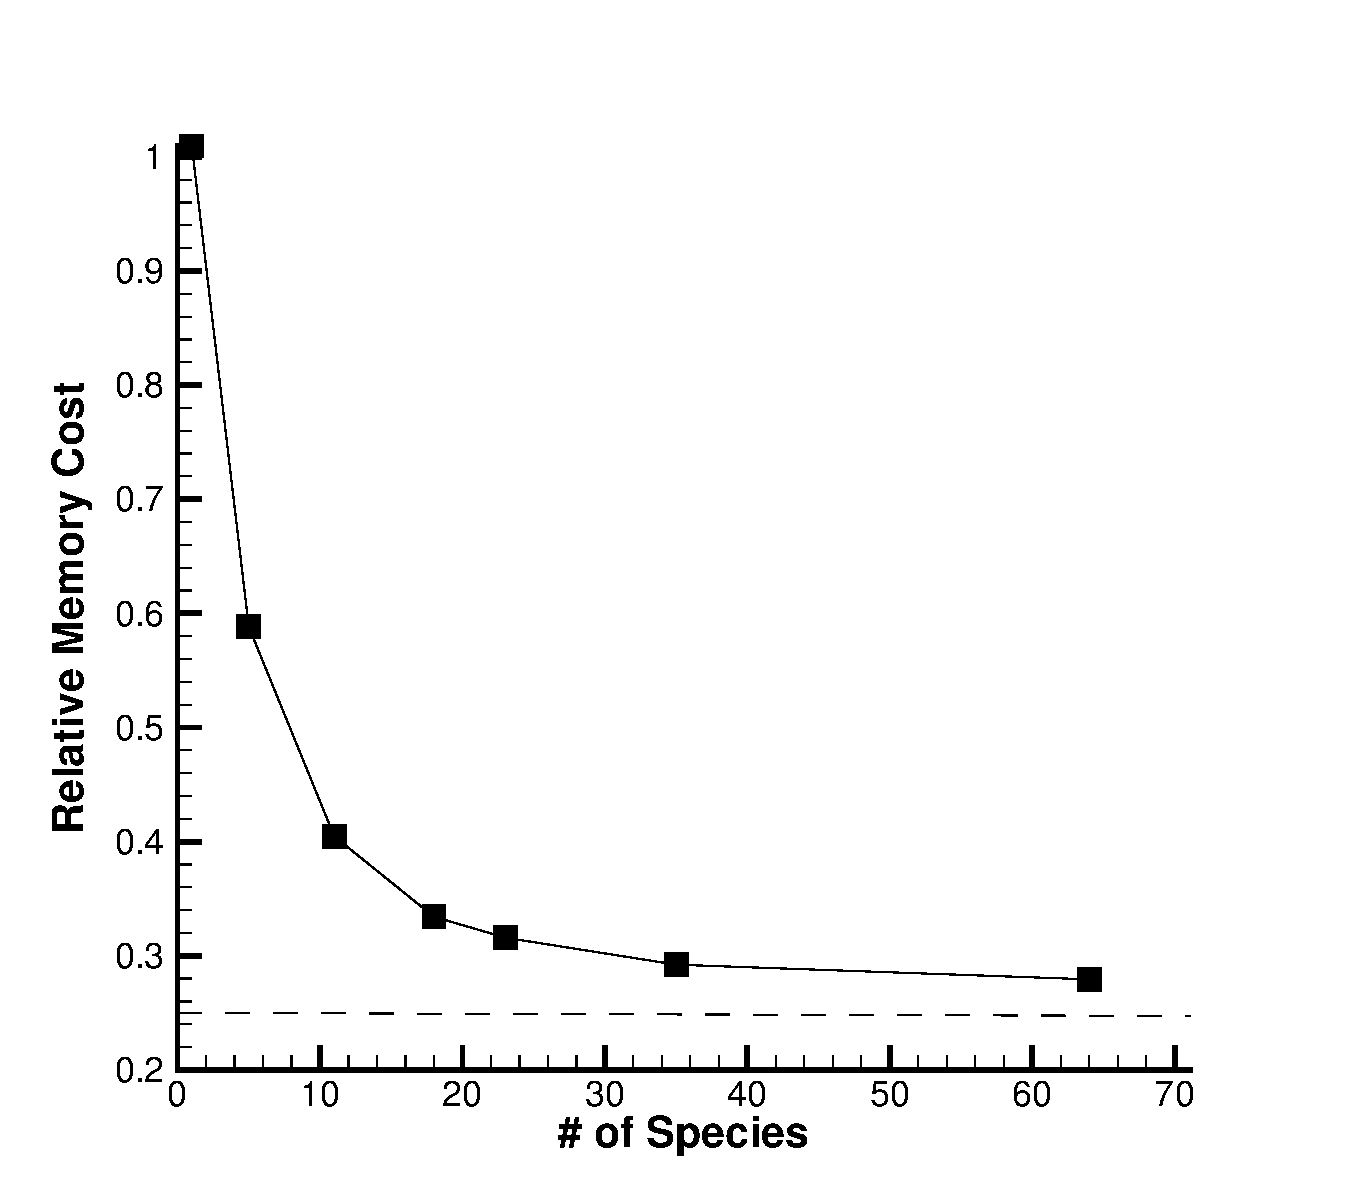
\includegraphics[width=0.45\textwidth]{figures/scitech/mem_req}
    \caption{Memory required convergence study.} 
    \vspace{-2em}
    \label{mem_req}
    \end{center} 
\end{figure}
%------------------------------------------------------------------------------%
thus, the relative memory saved by using the decoupled scheme correctly
approaches a factor of 1/4.

\subsection{Cylinder - Computational Cost}
\label{sec:cylinder-comp-cost}

As stated before, the cost of solving the decoupled implicit system should scale
approximately linearly with the number of species, whereas the fully coupled
problem should scale quadratically; thus, the speedup of the implicit solve
should be approximately linear when comparing the decoupled and fully coupled
approaches.  Figure \ref{rel_speedup} shows this to be true for the cylinder test
case, but that the total speedup of the problem is less than that of just
the linear solve.
%------------------------------------------------------------------------------%
\begin{figure}[h]
  \centering
  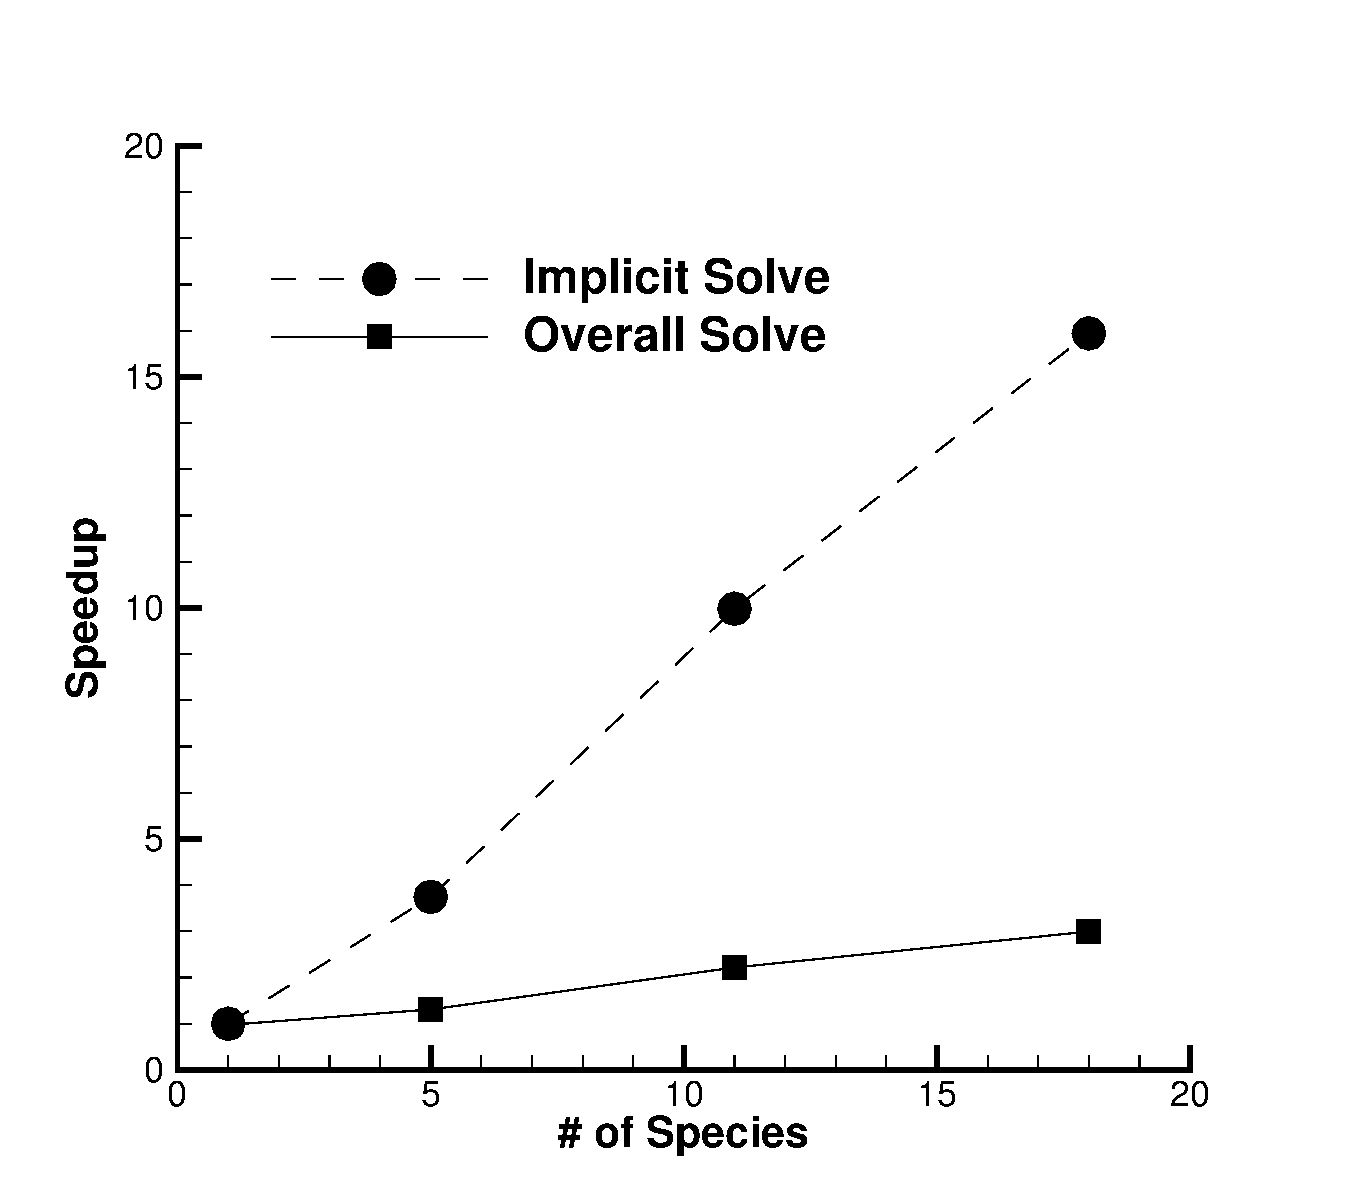
\includegraphics[width=0.45\textwidth]{figures/scitech/speedup} 
  \caption{ Relative speedup for the decoupled scheme vs. fully coupled scheme.}
  \label{rel_speedup} 
\end{figure}
%------------------------------------------------------------------------------%
The fact that the overall gains are not as large as those for the implicit
solve is due to Amdahl's law: the overall speedup is always limited by the
slowest component.  There are many other factors that scale with the number of
species, especially calculating the species source term and its linearization.
%------------------------------------------------------------------------------%
\begin{figure}[h]
  \centering
  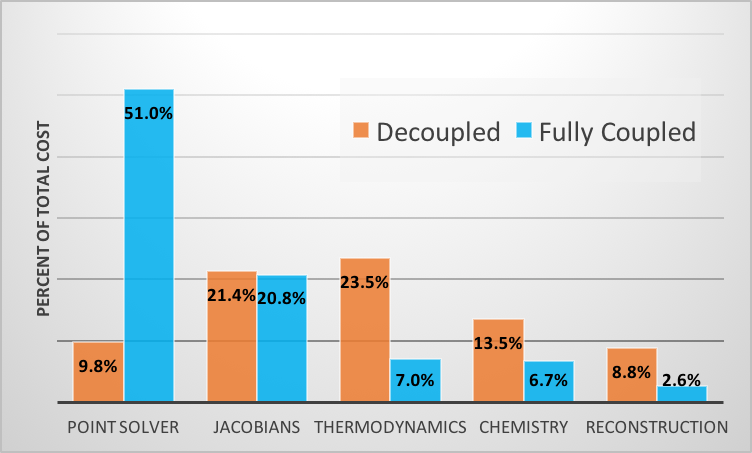
\includegraphics[width=0.5\textwidth]{figures/flow-efficiency/percent-cost.png}
  \caption{Relative cost of flow solver components for 11-species.}
  \label{fig:percent-cost-cyl}
\end{figure}
%------------------------------------------------------------------------------%
\fref{fig:percent-cost-cyl} shows that Jacobian evaluations and computing the
thermo-chemical state have superseded the linear solver as the dominant cost of
the simulation.  The overall speedup of the decoupled scheme over the fully
coupled scheme is constrained by these, and also highlights the sensitivity to
the Jacobian evaluation frequency.  When the non-linear update is rapidly
converging the residuals, the Jacobian is usually updated only one every 10
iterations.  Likewise, when the non-linear update is not resulting a sustained
residual decrease the Jacobian is updated every iteration.  This has a large
effect on relative computational efficiency, and poorly converging solutions can
be expected to show less relative speedup between the fully coupled and
decoupled schemes.

\section{15 km/s Flow over Spherically-Capped Cone}
\label{sec:15-kps-sphere-cone}

To ensure that the decoupled scheme is robust and accurate at higher velocities, both the
fully coupled and decoupled approaches were run on a sphere-cone geometry
identical to that presented by Candler et al. \cite{candler} (10 cm nose
radius, 1.1 m length, 8$^o$ cone angle).  For this case, a simple 64$\times$64
hexahedra grid was constructed, and freestream conditions were set as
$V_{\infty} = 15000\ m/s$, $\rho_{\infty}=0.001\ kg/m^3$, $T_\infty = 200\ K$.
Due to the large reaction rates during the transients at startup, when the
stagnation temperatures are very high, it was necessary to employ the scaling
factor, $\omega_r$ in order to ramp the magnitude of chemical source term.
Ramping was only required in the first 500 iterations, and no scaling was
performed on the source term when the solution was well with the radius of
convergence.

\subsection{Sphere-Cone - Verification of Implementation} 

As with the cylinder test case, the surface pressure and temperature were used
as metrics to determine that both the decoupled and fully coupled approaches
give the same answer when converged to steady-state. The species composition
consisted of N, $\text{N}_2$, O, $\text{O}_2$, NO, N$^+$, $\text{N}_2^+$, O$^+$,
$\text{O}_2^+$, NO$^+$, and electrons, with 22 possible reactions. Figure
\ref{cone_predictions} shows that both methods again yield similar results, and
the high stagnation temperature indicates that this is an inviscid,
one-temperature simulation.  This demonstrates that the decoupled approach is
able to converge to the same solution as the fully coupled solution, in spite of
the chemical reactions proceeding very rapidly due to a high stagnation
temperature.

%------------------------------------------------------------------------------%
\begin{figure}
	\centering
	\begin{subfigure}[b]{0.4\textwidth}
		\centering
		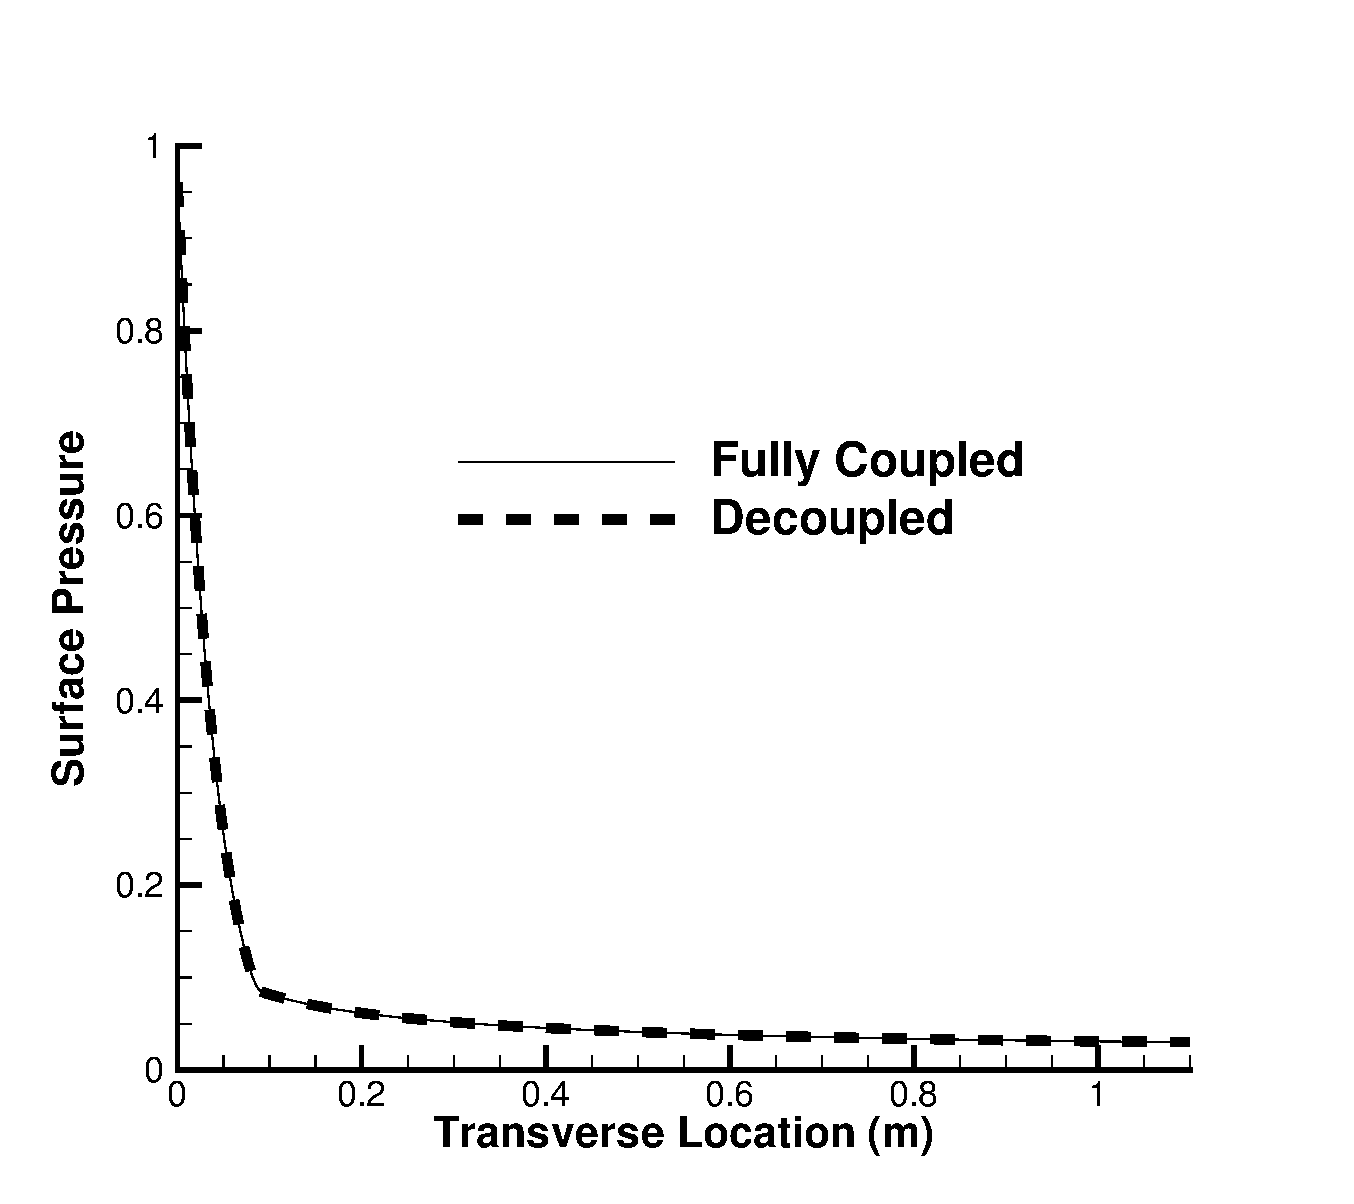
\includegraphics[width=\textwidth]{figures/scitech/surface_pressure_cone}
		\caption{Surface pressure}
		\label{cone_pressure}
	\end{subfigure}
	\begin{subfigure}[b]{0.4\textwidth}
		\centering
		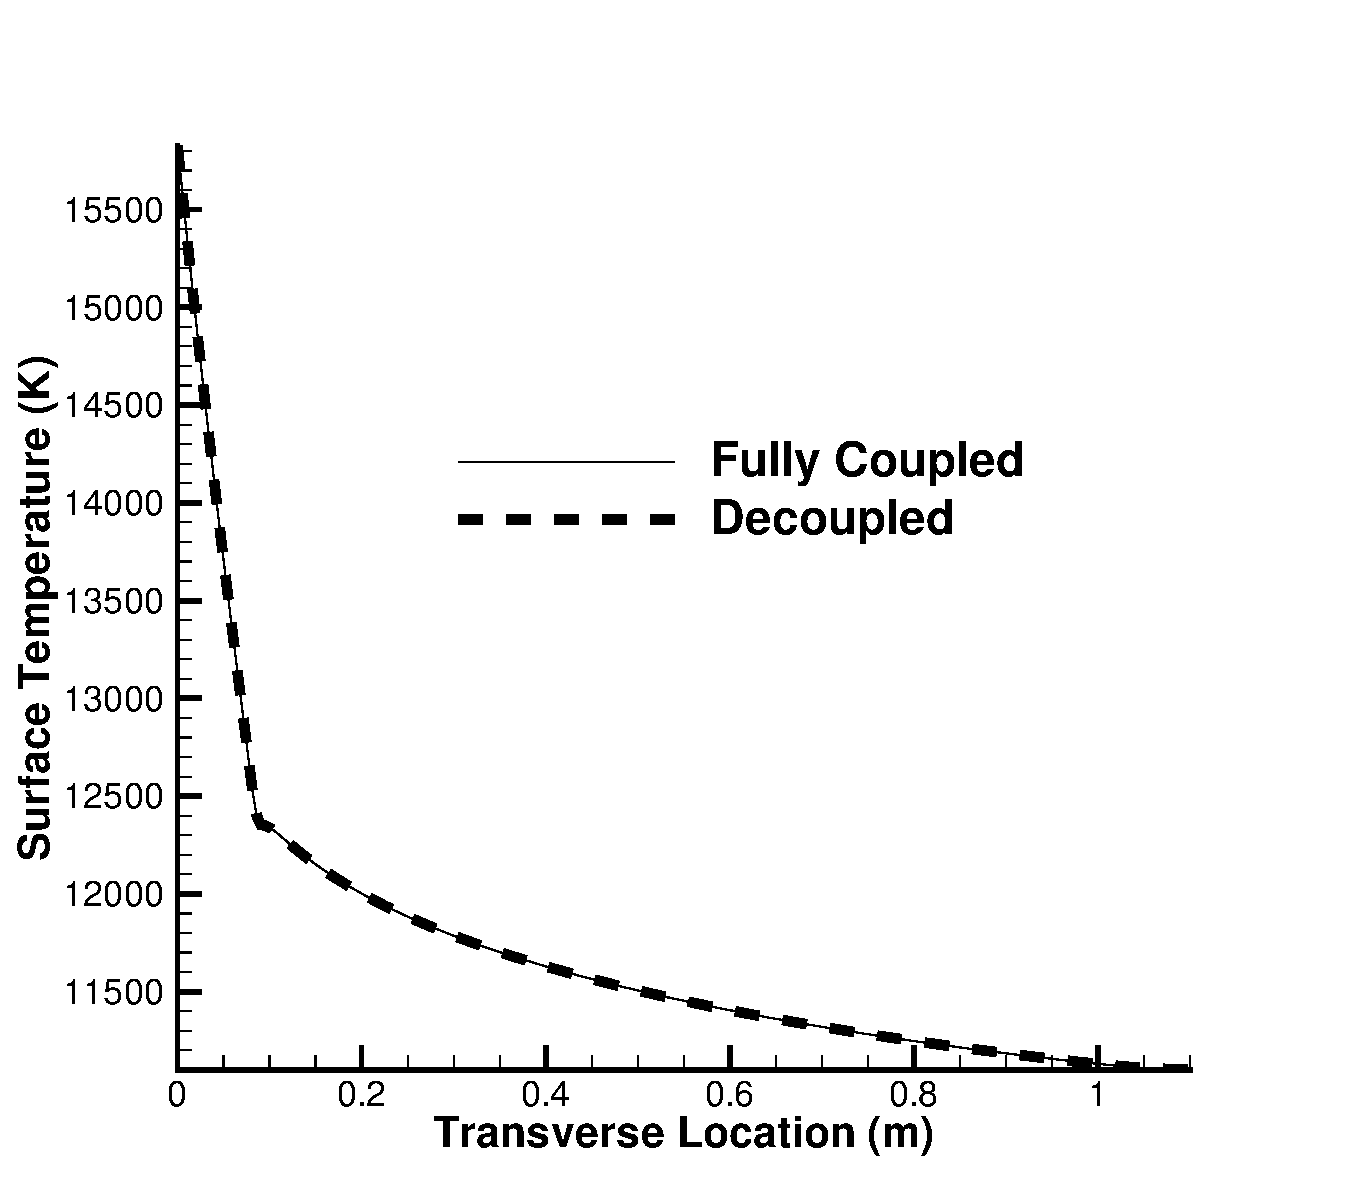
\includegraphics[width=\textwidth]{figures/scitech/surface_temperature_cone}
		\caption{Surface temperature}
		\label{cone_temp}
	\end{subfigure}
  \caption{Sphere-cone predicted quantities.}
  \label{cone_predictions}
\end{figure}
%------------------------------------------------------------------------------%

\subsection{Sphere-Cone - Convergence Quality}

The limits on the stability of the decoupled scheme derives from introducing
explicitness in creating and destroying species.  By scaling the magnitude of
the chemical source term during the transient phase of the solve, this
instability can be mitigated, and the convergence of decoupled scheme approaches
that of the fully coupled scheme. Scaling of chemical source term was done
identically between the decoupled and fully coupled scheme by ramping the
factor $\omega$ from 0.001 to 1.0 over the first 500 timesteps. Figure
\ref{cone_convergence} shows that the convergence of both schemes progresses
nearly identically, with the decoupled scheme converging in significantly less
computational time and, interestingly, fewer timesteps.
%------------------------------------------------------------------------------%
\begin{figure}
	\centering
	\begin{subfigure}[b]{0.45\textwidth}
		\centering
    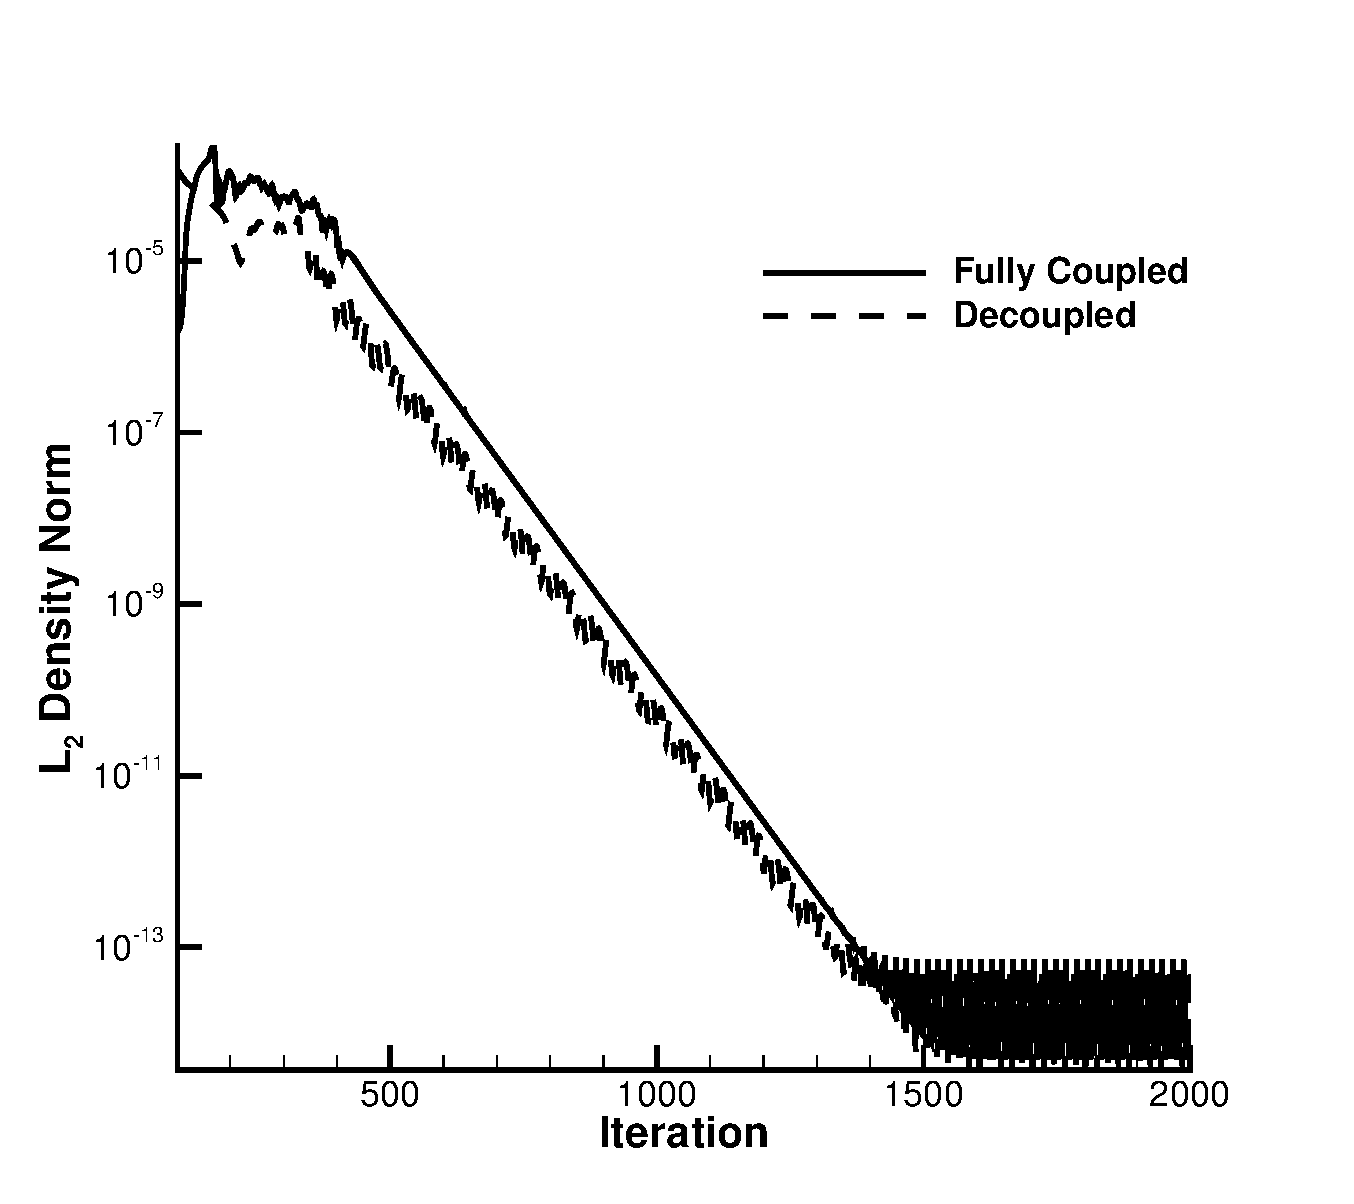
\includegraphics[width=\textwidth]{figures/scitech/cone_iteration}
		\caption{Iterations to convergence}
		\label{cone_iterations}
	\end{subfigure}
	\begin{subfigure}[b]{0.45\textwidth}
		\centering
		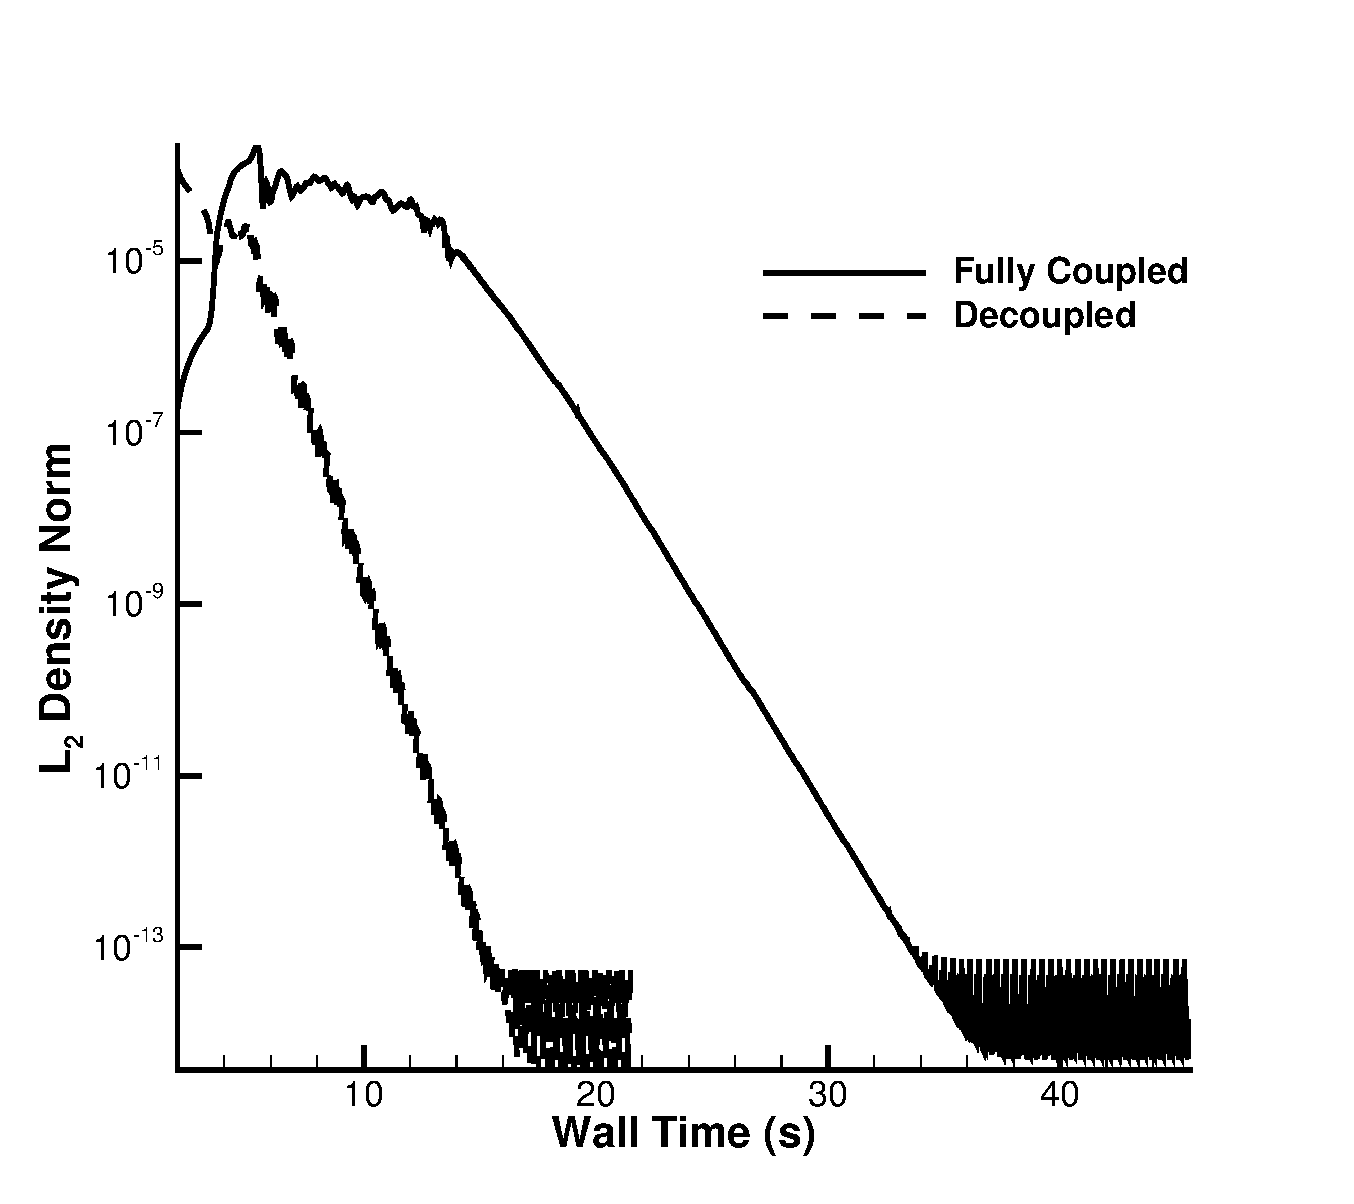
\includegraphics[width=\textwidth]{figures/scitech/cone_walltime}
    \caption{Computational time to convergence}
		\label{cone_walltime}
	\end{subfigure}
  \caption{Sphere-cone convergence details.}
  \label{cone_convergence}
\end{figure}
%------------------------------------------------------------------------------%
This demonstrates that the decoupled scheme has significant potential to
improve the efficiency of high-velocity simulations, and that the stiffness of
the source term can be overcome in the presence of large chemical reaction
rates.

\subsection{Sphere Cone - Convergence Improvement with Exact First-Order Linearizations}
\label{sec:sphere-cone-exact-approx-convergence}

An important benefit of implementing an adjoint solver in FUN3D derives from the
requirement of exact linearizations, because the linearizations needed to form
the residual in the adjoint solver can be reused by the flow solver.
Due to the high storage requirements associated with exactly linearizing the
gradient terms in the reconstruction, an approximate Jacobian is used in the
flow solver.  This approximate Jacobian consists of linearizations of the
first-order scheme, as is used to solve the governing equations via defect
correction.  Previously, the reacting gas path employed a Jacobian also, that
approximated the linearizations of the Roe FDS scheme\cite{gnoffo-tp} as
%------------------------------------------------------------------------------%
\begin{equation}
  \rdiff{}{\mU} = 
  \frac{1}{2} \left( \rdiff{c}{\mU} + \rdiff{\tilde{c}}{\mU} \right)
  \label{approx-roe-jac}
\end{equation}
%------------------------------------------------------------------------------%
where $\rdiff{c}{\mU}$ is the linearization of the convective portion of the Roe
FDS scheme, and $\rdiff{\tilde{c}}{\mU}$ is the approximation to the dissipation
term in the Roe RDS scheme, formed by evaluating $\rdiff{c}{\mU}$ with Roe
averaged quantities.  This approximation has been is used by others
\cite{rinaldi2014exact} to mitigate the development time of implementing an
exact linearization of the dissipation term in the Roe FDS scheme, as well the
large computational cost in computing those linearizations at each Jacobian
update.

To demonstrate any benefit of the exact linearization of the Roe FDS scheme on
iterative convergence of the flow solver, the sphere cone case was converged
using both the Jacobian employing exact linearizations of the Roe FDS scheme
flux, and the Jacobian employing the approximation in \eref{approx-roe-jac}.
%------------------------------------------------------------------------------%
\begin{figure}[h]
  \centering
  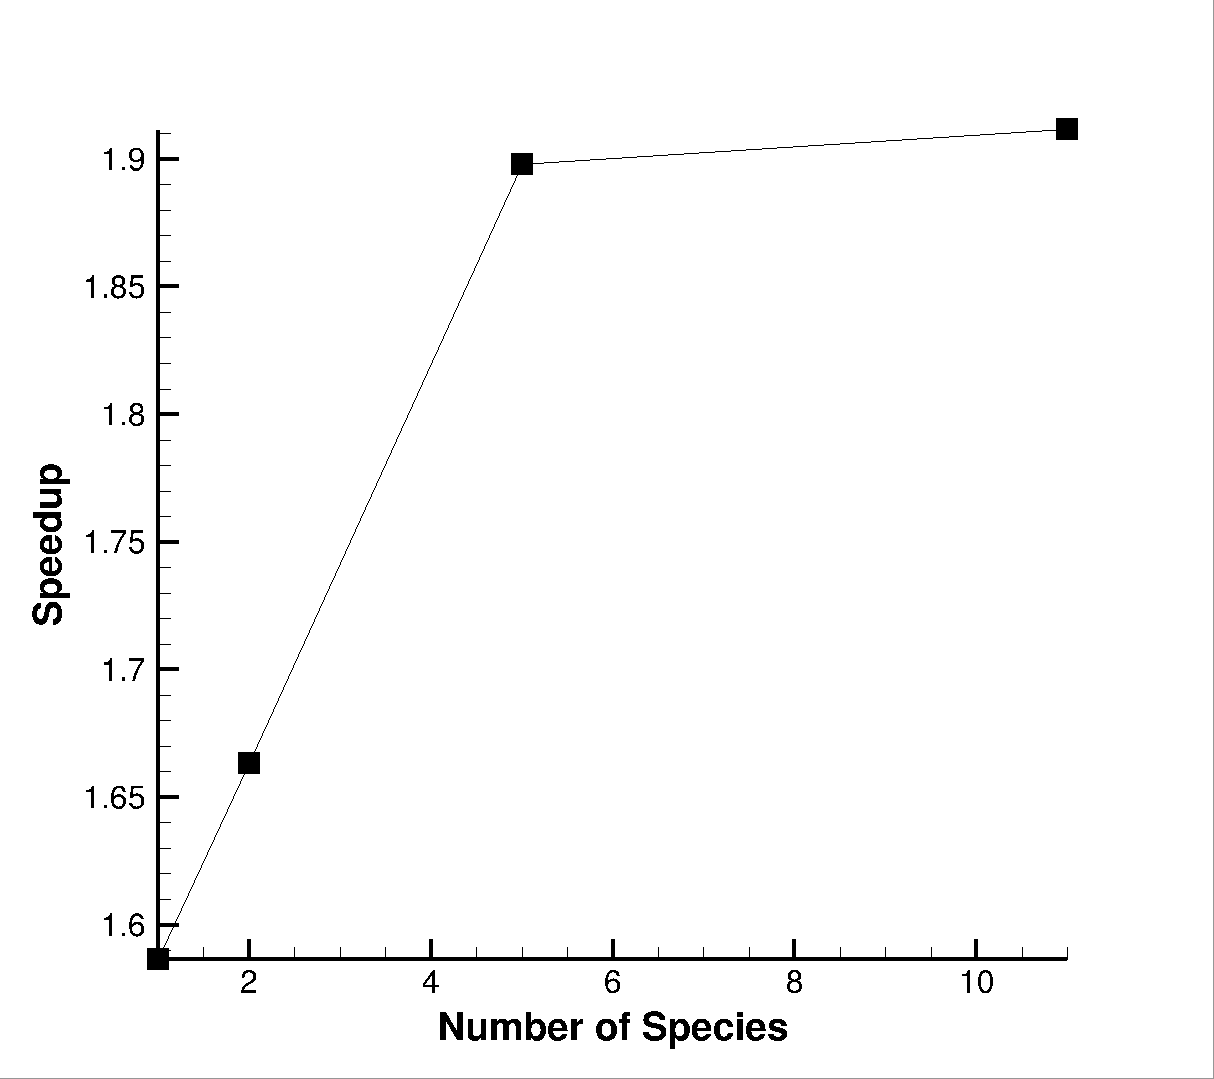
\includegraphics[width=0.5\textwidth]{figures/flow-efficiency/exact-approx-speedup.png}
  \caption{Relative speedup using exact linearizations.}
  \label{fig:exact-approx-speedup}
\end{figure}
%------------------------------------------------------------------------------%
\fref{fig:exact-approx-speedup} shows that up to a five-species air mixture, the
convergence to steady state is completed in $58\%$ to $90\%$ less simulation
time.  For the 11 species air mixture, involving ionization, the speed up
promptly plateaus, as the additional costs incurred by computing the exact
linearizations supersede the improved iterative convergence.  It can be inferred
from \fref{fig:exact-approx-speedup} that the improvements compounded by the
decoupled scheme, which affords iterative converge similar to the exact fully
coupled scheme, will be significantly faster than the baseline scheme that was
originally implemented in the reacting gas path of FUN3D.

\section{Re-entry Vehicle with Retro-Firing Annular Jet}

The demonstration problem presented in \crefs{chapter-five}{chapter-six}
presents the most challenging problem for the decoupled scheme, due to the
Hydrogen-air combustion.  To verify that the solution is not effected by
employing the decoupled scheme over the fully coupled scheme, the comparison is
made between solutions of the decoupled and fully coupled flow solvers on the
cost function component quantities in \sref{cost-func-components}.  The
freestream conditions in \tref{tab:flow-conditions} were used for this
comparison, along with the plenum conditions in \tref{tab:plenum-conditions}.

\subsection{Annular Jet: Verification of Implementation}
\label{sec:annular-jet-flow-verify}

To determine consistency between the fully coupled and decoupled schemes, the
surface temperature RMS, $T_{RMS}$, and mass flow rate, $\massflow$, were
computed and compared.  Because of the flux limiter sensitivity and poor
relative convergence with finite-rate chemistry discussed in
\sref{sec:frozen-limiter}, the comparison was made for both frozen flow and
flow in chemical non-equilibrium.
%------------------------------------------------------------------------------%
\begin{table}
  \centering
  \begin{tabular}{c|c|c|c}
    Quantity & Decoupled & Fully Coupled & Relative Difference \\
    \hline
    $\massflow$ & 0.8450858226893225E-03 & 0.8450858226893034E-03 & 2.26E-14 \\
    $T_{RMS}$   & 0.1508600871984388E+04 & 0.1508600871984388E+04 & 0
  \end{tabular}
  \caption{Difference with frozen chemistry.}
  \label{tab:srp-frozen-flow-diff}
\end{table}
%------------------------------------------------------------------------------%
\tref{tab:srp-frozen-flow-diff} shows that, for frozen chemistry, the decoupled
and fully coupled schemes match discretely for surface temperature, and to
within approximately machine precision for the mass flow rate through the
plenum.  The residual was less than $10^{-16}$ for all equations in this
comparison, and only the last digit of both quantities in
\tref{tab:srp-frozen-flow-diff} were changing by the end of the solution.
%------------------------------------------------------------------------------%
\begin{table}
  \centering
  \begin{tabular}{c|c|c|c}
    Quantity & Decoupled & Fully Coupled & Relative Difference \\
    \hline
    $\massflow$ & 0.8448720721551258E-03 & 0.8448720721551088E-03 & 2.01E-14 \\
    $T_{RMS}$   & 0.1545729169703027E+04 & 0.1545720949811712E+04 & 5.32E-06
  \end{tabular}
  \caption{Difference with finite-rate chemistry.}
  \label{tab:srp-chem-flow-diff}
\end{table}
%------------------------------------------------------------------------------%
\tref{tab:srp-chem-flow-diff} shows, for reacting chemistry, similar agreement
with regard to the plenum mass flow rate, but poorer agreement of the surface
temperature. Given the varying degrees of convergence shown in
\fref{fig:chem-res-comp}, this difference in surface temperature is not
surprising. At the point the convergence stall, with the residual of all
equations hanging at $\sim 10^{-8}$, only the last nine digits were still
changing.  This indicates that improving the conditioning of the problem, in
order to enable further converge of the flow equation residuals to machine zero,
would likely decrease the relative difference between the fully coupled and
decoupled flow solver schemes.  For engineering applications this difference is
trivial and it has only minimal impact, if any, on the design optimization
procedure.  The effect of the flux limiter sensitivity is much greater on the
design optimization procedure, and it was found that the using the decoupled
scheme or the fully-coupled scheme in the optimization from \cref{chapter-five}
converged to the same result if the limiter fields were made identical between
the schemes.

\subsection{Annular Jet: Convergence Quality}

Due to startup transients, where reaction rates grew very large as nearly all
$H_2$ and $O_2$, and most of $N_2$, dissociated near the stagnation region, the
source term scaling factor, $\omega_r$, was employed for this problem to
maintain stability.  It was empirically determined that the source term scaling
could be removed within the first third of the way to convergence for this
problem.  

%------------------------------------------------------------------------------%
\begin{figure}[h]
  \centering
	\begin{subfigure}[b]{0.45\textwidth}
    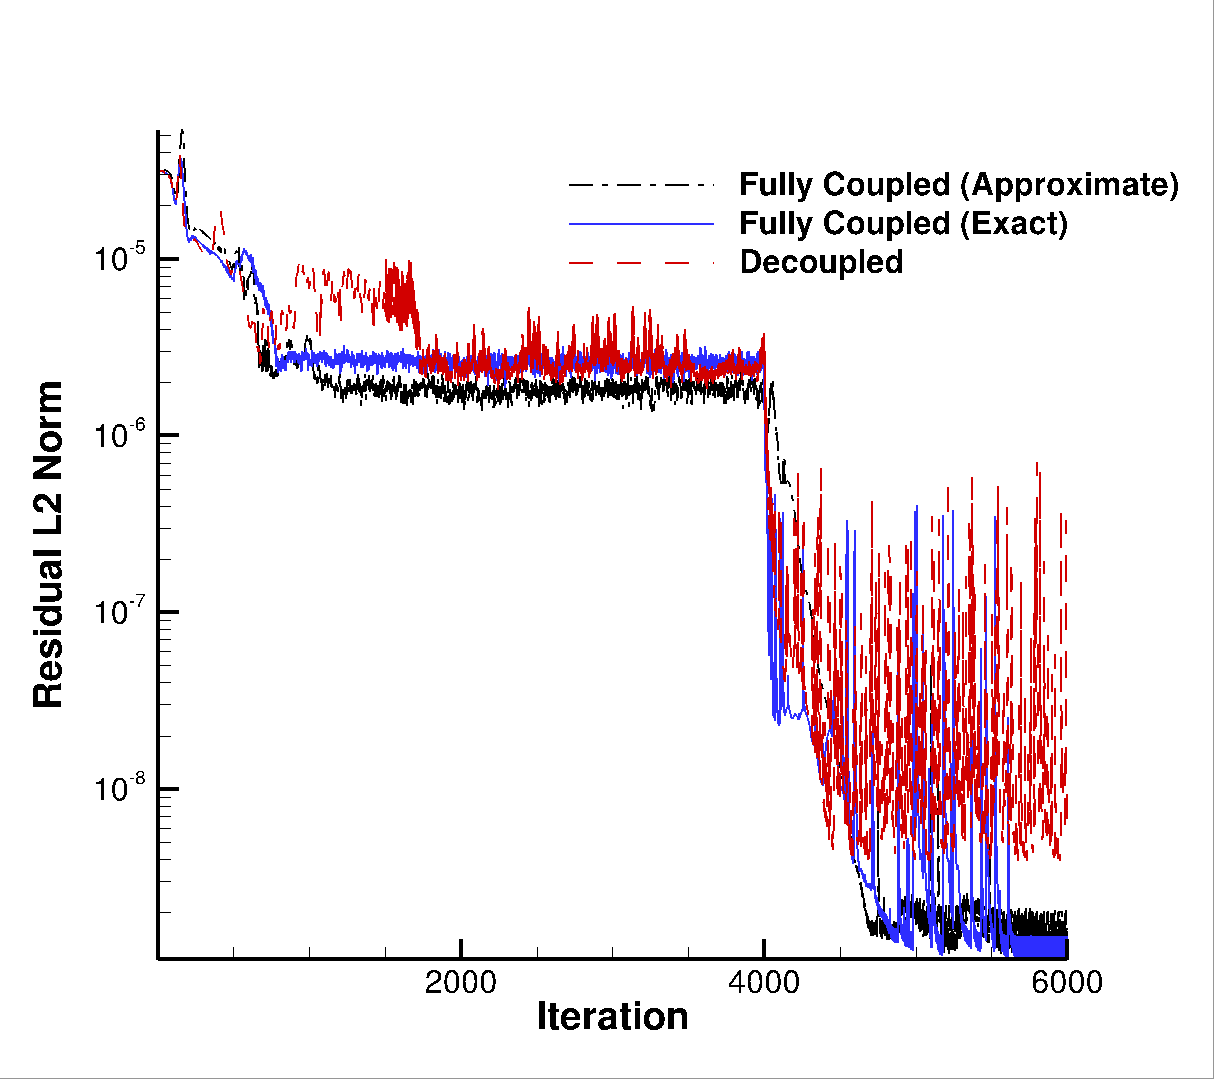
\includegraphics[width=\textwidth]{figures/flow-efficiency/dc-gfc-res-chem.png}
    \caption{Finite-rate chemistry}
    \label{fig:srp-dc-gfc-res-frozen}
  \end{subfigure}
	\begin{subfigure}[b]{0.45\textwidth}
    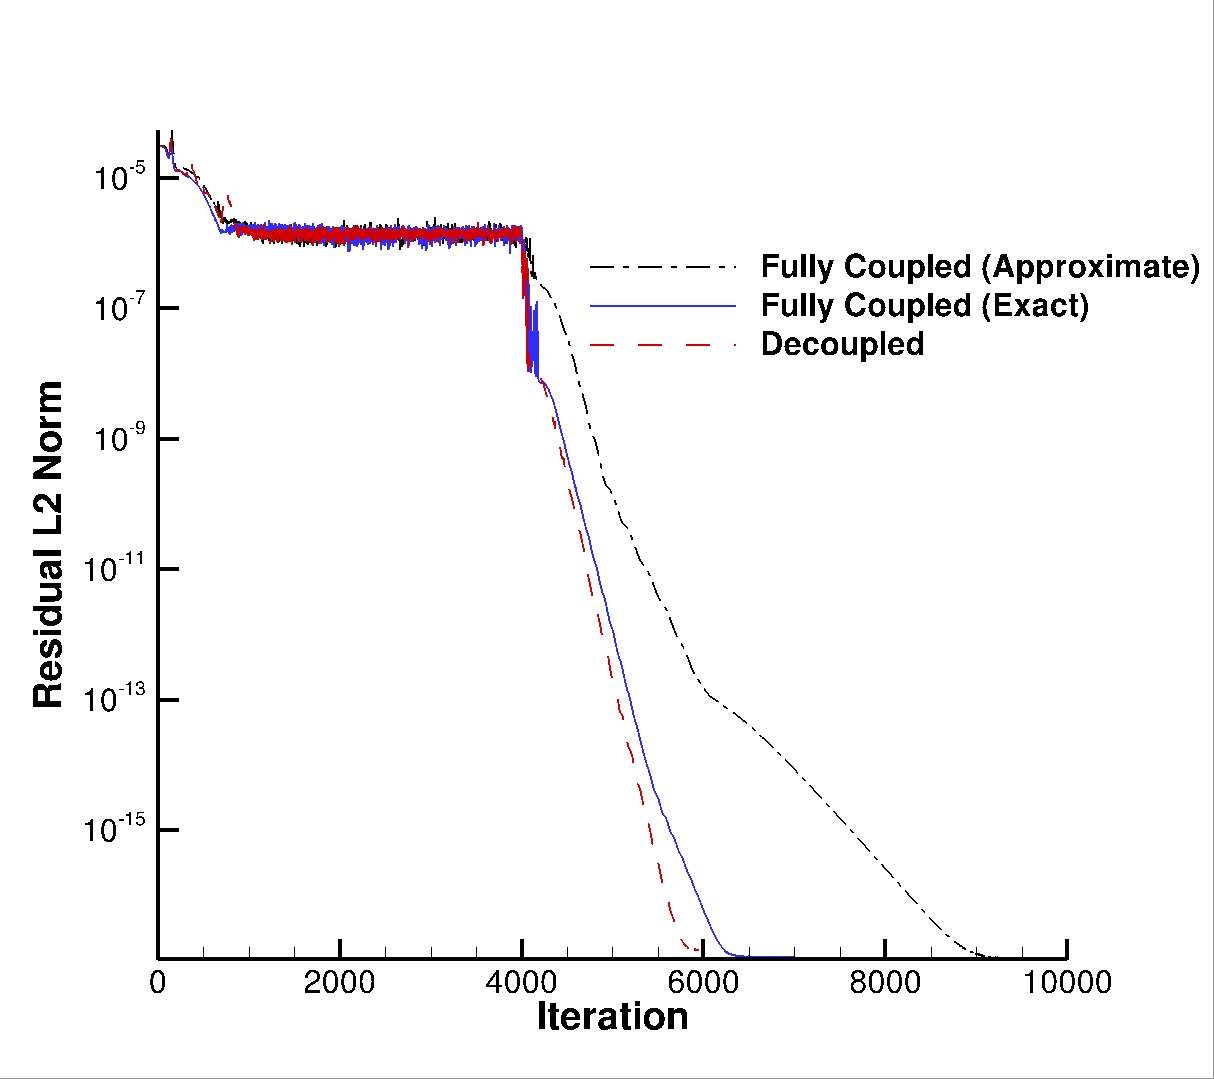
\includegraphics[width=\textwidth]{figures/flow-efficiency/dc-gfc-res-frozen.png}
    \caption{Frozen chemistry}
    \label{fig:srp-dc-gfc-res-chem}
  \end{subfigure}
  \caption{Second-order residual convergence history.}
  \label{fig:srp-dc-gfc-res}
\end{figure}
%------------------------------------------------------------------------------%
\fref{fig:srp-dc-gfc-res} shows a comparison of the residual convergence for the
fully coupled schemes, with exact first-order linearizations and the
approximations described in \sref{sec:sphere-cone-exact-approx-convergence}, and
the decoupled scheme.  The comparing
\frefs{fig:srp-dc-gfc-res-frozen}{fig:srp-dc-gfc-res-chem}, there is a stark
difference both the minimum residual convergence and the ``smoothness'' of the
convergence profile.  When the no chemical source terms are present (frozen
flow), the flow equation residuals are able to be converged to $ < 10^{-16}$,
with very few high-frequency errors encountered after the limiter is frozen at
4000 iterations.  When chemistry is engaged, the convergence of the flow
equation residuals stalls at approximately $10^{-8}$, and there are a large
number of high-frequency errors in the solution updates after the limiter is
frozen, due to the frozen limiter needing to be re-evaluated.
\fref{fig:srp-dc-gfc-res-chem} shows that the decoupled scheme is more
sensitive to the frozen limiter than either of the fully coupled schemes.  This
is not overly surprising, since the re-evaluation of the flux limiter is
sensitive to subtle changes in the species densities, and the decoupled
scheme Jacobians have a large number of approximations with regard to species
density linearizations.  As show in \sref{sec:annular-jet-flow-verify}, the
impact of this poor convergence quality on the quantities of interest is
minimal, and this degree of convergence is more than sufficient to obtain the
sensitivity gradients required in design optimization.

\subsection{Annular Jet: Relative Speedup}

The computational cost of decoupled scheme and fully coupled scheme with exact
first-order linearizations is compared to the previously implemented fully coupled
scheme with approximate first-order linearizations.
For flow with frozen chemistry, show in \fref{fig:srp-dc-gfc-res-frozen},
the solution is considered converged when the flow residual $L_2$ norm is less
than $10^{-16}$, and the relative speedup is shown in
\tref{tab:srp-rel-speedup-frozen}
%------------------------------------------------------------------------------%
\begin{table}[h]
  \centering
  \begin{tabular}{c|c|c}
    Scheme & Time (s) & Speedup \\
    \hline
    Fully Coupled (Approximate) & 348.6 & 1.0 (baseline) \\
    Fully Coupled (Exact)       & 265.6 & 1.31 \\
    Decoupled                   & 138.7 & 2.51
  \end{tabular}
  \caption{Relative speedup for frozen chemistry.}
  \label{tab:srp-rel-speedup-frozen}
\end{table}
%------------------------------------------------------------------------------%
The decoupled scheme is considerably faster than either of the two fully coupled
schemes, and the improved iterative convergence afforded by the exact
linearizations prove valuable to the fully coupled scheme for this case, where
the residuals can be converged an additional 10 orders of magnitude after the
limiter is frozen.  Determining the relative speedup is difficult for the
schemes in \fref{fig:srp-dc-gfc-res-chem}, where finite-rate chemistry is
engaged, due to noise in the convergence history.  Because of this, total
solution time is used in lieu of a residual convergence level to compute the
relative speedup in \tref{tab:srp-rel-speedup-chem}
%------------------------------------------------------------------------------%
\begin{table}[h]
  \centering
  \begin{tabular}{c|c|c}
    Scheme & Time (s) & Speedup \\
    \hline
    Fully Coupled (Exact)       & 280.6 & 1.0 (baseline) \\
    Fully Coupled (Approximate) & 270.4 & 1.04 \\
    Decoupled                   & 168.6 & 1.66
  \end{tabular}
  \caption{Relative speedup for finite-rate chemistry.}
  \label{tab:srp-rel-speedup-chem}
\end{table}
%------------------------------------------------------------------------------%
The gains associated with chemistry engaged are significantly less than those
with frozen chemistry for this annular jet case.  Due to stalled convergence,
there is no clear advantage of using exact linearizations over approximate
linearizations in the fully coupled scheme, although the relative savings of use
approximate linearizations are almost negligible ($4\%$).  The decoupled scheme
is 66\% faster than the exact, fully coupled scheme, and the difference between
this result and the frozen flow result is the poorer iterative convergence
quality.  As discussed in \sref{sec:cylinder-comp-cost}, the frequency of
the Jacobian evaluation is tied to the decrease in the residual from each
non-linear solution update.  Due to the poorer convergence seen in
\fref{fig:srp-dc-gfc-res-chem}, the Jacobian is reevaluated at each iteration.
This significantly diminishes the relative speedup of the decoupled scheme.
This causes the Jacobian update to become a bottleneck in computational time
required, and the additional cost of computing chemical source term and its
Jacobian at each timestep reduces the relative speedup further in comparison to
frozen flow.

